\documentclass[12pt,a4paper]{article}
\usepackage[utf8]{inputenc}
\usepackage{geometry}
\usepackage{graphicx}
\usepackage{amsmath} % for the "align" and "align*" environments
\graphicspath{ {images/} }



\geometry{legalpaper, portrait, margin=1.25in}

\newcommand*\rfrac[2]{{}^{#1}\!/_{#2}}

\title{
    ECE454 Distributed Systems\\ 
    A2 Part a Answers
}
\author{
    Fasih Awan\\
    \texttt{20424848}
    \and
    Victor Lai\\
    \texttt{20426719}
    \and
    Aaron Morais\\
    \texttt{20413440}
}

\vfill

\date{
    June 12, 2015
}

\usepackage{enumitem}

\begin{document}

\maketitle
\clearpage

\section{~}

Assume the following: one-way network delay of $100ms$ between client and server, and $50ms$ processing delay in the service handler.

\begin{enumerate}[label=(\alph*)]

\item \textbf{Estimate the latency of a synchronous RPC, as illustrated in slide 5 of lecture module 04}

The client sends a synchronous request to the server, invoking a $100\ ms$ delay. The client blocks while the server processes the data for $50\ ms$. The server sends the data, and the client receives the data after another $100\ ms$ delay. This means the latency is $100\ ms + 50\ ms + 100\ ms = 250\ ms$.

\item \textbf{Estimate the latency of an asynchronous RPC, as illustrated in slide 15 of lecture module 04}

The client sends an asynchronous request to the server, invoking a $100\ ms$ delay. The server immediately sends an accept to the client, which the client will receive in $100\ ms$. The server also begins processing the data for $50\ ms$. The server completes the processing before the client receives the accept request and sends the results back to client, which takes another $100\ ms$. So $50\ ms$ after the client receives the accept request, the client also receives the results. So the total latency is still $100\ ms + 50\ ms + 100\ ms = 250\ ms$ as well. 

\item \textbf{Estimate the maximum throughput (RPCs per second) for synchronous calls if the service handler runs inside THsHaServer with a pool of four worker threads on an eight-core processor}

A THsHaServer has 1 network I/O thread and 4 worker threads. Because the server runs on an eight-core processor, we assume that every thread can run on its own core, so we can simplify by not worrying about thread scheduling.

Because each thread can run on its own core, as long as we have one worker thread available to either accept or return a response at all times, the network thread can be used for another 100ms, in which case any current worker thread processing will have been completed. If we interleave the requests and responses optimally (in the case of maximum throughput), we can bypass the costs of the worker thread processing.

Because we don't have to worry about the processing delay, all of our delay will be due to the 1 network I/O thread. So we are limited by how fast the network thread can accept and return the result. It takes $100\ ms$ to accept and $100\ ms$ to return the result, so $100\ ms + 100\ ms = 200\ ms$ to process 1 request.

\begin{align*}
 \frac{1\ s}{\rfrac{200\ ms}{request}} = 5\ requests
\end{align*}

So we can process a maximum of 5 requests per second.

\end{enumerate}



\clearpage

\section{~}

Consider NTP as described in lecture module 06a. Suppose that the actual offset of B relative to A is $1ms$, and that the network delays $dT_{req}$ and $dT_{res}$ are independent random variables distributed uniformly over the interval $[8ms, 12ms]$.

\begin{equation*}
    \begin{split}
        X = T_2 - T_1 &= dT_{req} \in [8, 12]\ ms \\
        Y = T_4 - T_3 &= dT_{res} \in [8, 12]\ ms \\ 
        \theta_{real} &= 1\ ms \\
    \end{split}
\end{equation*}

\begin{enumerate}[label=(\alph*)]

\item \textbf{Determine the probability distribution of $\theta$, the estimate of the offset of host B relative to host A}
    
    \begin{equation*}
        \begin{split}
            \theta_{est} &= \frac{(T_2-T_1) - (T_4-T_3)}{2} \\
            Z &= \frac{X - Y}{2} \\
            X &= 2Z + Y \\
        \end{split}
    \end{equation*}
    \begin{equation*}
        \begin{split}
            \text{Let $f_x$ be the density function of X} \\
            \text{Let $f_y$ be the density function of Y} \\
            \text{Let $f_z$ be the density function of Z} \\
        \end{split}
    \end{equation*}
    \begin{equation*}
        \begin{split}
            f_x(x) = f_y(y) &= 
            \begin{cases}
                  \frac{1}{4}   & 8 \leq x \leq 12 \\
                  0             & otherwise
            \end{cases} \\
        \end{split}
    \end{equation*}
    
    \begin{equation*}
        \begin{split}
            f_z(z) &= \int_{-\infty}^{+\infty} f_x(x) f_y(y) dy \\
            f_z(z) &= \int_{-\infty}^{+\infty} f_x(2z + y) f_y(y) dy \\
            f_z(z) &= \frac{1}{4} \int_{8}^{12} f_x(2z + y) dy \\
            t &= 2z + y \\
            dt &= dy \\
            y &= 8 \implies t = 2z + 8 \\
            y &= 12  \implies t = 2z + 12 \\
            f_z(z) &= \frac{1}{4} \int_{2z+8}^{2z+12} f_x(t) dt \\
        \end{split}
    \end{equation*}
    \begin{equation*}
        \begin{split}
            \text{The range of $t$ is $8 \leq t \leq 12$, otherwise $f_x(t) = 0$.} \\
        \end{split}
    \end{equation*}
    \begin{equation*}
        \begin{split}
            f_z(z) &= \frac{1}{4} \int_{8}^{12+2z} \frac{1}{4} dt  = \frac{(2z + 12) - 8}{16} = \frac{2z + 4}{16}\ \text{for $-2 \leq z \leq 0$} \\
            f_z(z) &= \frac{1}{4} \int_{2z+8}^{12} \frac{1}{4} dt = \frac{12 - (2z + 8)}{16} = \frac{4 - 2z}{16}\ \text{for $0 \leq z \leq 2$} \\
            f_z(z) &=
            \begin{cases}
                  \frac{2z + 4}{16}    & -2 \leq z \leq 0 \\
                  \frac{4 - 2z}{16}    & 0 \leq z \leq 2 \\
                  0         & otherwise \\
            \end{cases} \\
        \end{split}
    \end{equation*}

\clearpage
\item \textbf{Determine the probability distribution of $\delta$, the estimate of the network delay between A and B}

    \begin{equation*}
        \begin{split}
            \delta_{est} &= \frac{(T_4 - T_1) - (T_3 - T_2)}{2} \\
            \delta_{est} &= \frac{(T_2 - T_1) + (T_4 - T_3)}{2} \\
            2Z &= X + Y \\
            X &= 2Z - Y \\
        \end{split}
    \end{equation*}
    \begin{equation*}
        \begin{split}
            \text{Let $f_x$ be the density function of X} \\
            \text{Let $f_y$ be the density function of Y} \\
            \text{Let $f_z$ be the density function of Z} \\
        \end{split}
    \end{equation*}
    \begin{equation*}
        \begin{split}
            f_x(x) = f_y(y) &= 
            \begin{cases}
                  \frac{1}{4}   & 8 \leq x \leq 12 \\
                  0             & otherwise
            \end{cases} \\
        \end{split}
    \end{equation*}
    
    \begin{equation*}
        \begin{split}
            f_z(z) &= \int_{-\infty}^{+\infty} f_x(x) f_y(y) dy \\
            f_z(z) &= \int_{-\infty}^{+\infty} f_x(2z - y) f_y(y) dy \\
            f_z(z) &= \int_{8}^{12} f_x(2z - y) \frac{1}{4} dy \\
            t &= 2z - y \\
            dt &= -dy \\
            y &= 8 \implies t = 2z - 8 \\
            y &= 12  \implies t = 2z - 12 \\
            f_z(z) &= - \frac{1}{4} \int_{2z-8}^{2z-12} f_x(t) dt \\
            f_z(z) &= \frac{1}{4} \int_{2z-12}^{2z-8} f_x(t) dt \\
        \end{split}
    \end{equation*}
    \begin{equation*}
        \begin{split}
            \text{The range of $t$ is $8 \leq t \leq 12$, otherwise $f_x(t) = 0$.} \\
        \end{split}
    \end{equation*}
    
    \begin{equation*}
        \begin{split}
            f_z(z) &= \frac{1}{4} \int_{8}^{2z-8} \frac{1}{4} dt     = \frac{12z - 8 - 8}{16} = \frac{2z - 16}{16} \ \text{for $8 \leq z \leq 10$} \\
            f_z(z) &= \frac{1}{4} \int_{2z-12}^{12} \frac{1}{4} dt   = \frac{12 - (2z - 12)}{16} = \frac{24 - 2z}{16} \ \text{for $10 \leq z \leq 12$} \\
            f_z(z) &= 
            \begin{cases}
                  \frac{2z - 16}{16}    & 8 \leq z \leq 10 \\
                  \frac{24 - 2z}{16}    & 10 \leq z \leq 12 \\
                  0          & otherwise \\
            \end{cases} \\
        \end{split}
    \end{equation*}



\clearpage

\item \textbf{If NTP collects only one ($\theta$, $\delta$) pair, determine the probability that the estimated $\theta$ is in the interval [0.9ms,1.1ms]}

The probability density function of $\theta$ looks like this, centered around the origin.

    \begin{equation*}
        \begin{split}
            f_z(z) &=
            \begin{cases}
                  \frac{2z + 4}{16}    & -2 \leq z \leq 0 \\
                  \frac{4 - 2z}{16}    & 0 \leq z \leq 2 \\
                  0         & otherwise \\
            \end{cases} \\
        \end{split}
    \end{equation*}

The probability that the $\theta$ lies within [0.9, 1.1] would be the integral of this function over that range.

    \begin{equation*}
        \begin{split}
            f_z(0.9 \leq z \leq 1.1) &= \int_{0.9}^{1.1}f_z(z) dz \\
                                     &= \int_{0.9}^{1.1} \frac{4-2z}{16} dz \\
                                     &= \left[\frac{4z - z^2}{16}\right]|_{0.9}^{1.1} \\ 
                                     &= \frac{1}{16} \left(\left[4(1.1)-(1.1)^2\right] - \left[4(0.9)-(0.9)^2\right]\right) \\
                                     &= \frac{1}{16} \left(3.19 - 2.79\right) \\ 
                                     &= 0.025 \\
        \end{split}
    \end{equation*}
    
Therefore, the probability that $\theta$ lies within [0.9, 1.1] is 0.025, or 2.5\%.

\end{enumerate}

\section{~}


\begin{enumerate}[label=(\alph*)]
\item \textbf{List all the events that happen before the specific event with vector clock [A:blank, B:3, C:1].}


\begin{itemize}
\item \textbf{[ A:0, B:0, C:1 ]} 
\item \textbf{[ A:0, B:1, C:1 ]} 
\item \textbf{[ A:0, B:2, C:1 ]} 

\end{itemize}

\item \textbf{List all the events that happen after the specific event with vector clock [A:2, B:2, C:1].(Y “happens after” X if X happens before Y.)}

\begin{itemize}

\item \textbf{[ A:2, B:4, C:1 ]}
\item \textbf{[ A:2, B:5, C:1 ]}
\item \textbf{[ A:2, B:5, C:4 ]}
\item \textbf{[ A:2, B:5, C:5 ]}
\item \textbf{[ A:3, B:3, C:3 ]}
\item \textbf{[ A:3, B:5, C:5 ]} 

\end{itemize}

\item The events that are concurrent with [A:3, B:3, C:3] are:

\begin{itemize}
\item \textbf{[A:2, B:4, C:1]}
\item \textbf{[A:2, B:5, C:1]}
\item \textbf{[A:2, B:5, C:4]}
\item \textbf{[A:2, B:5, C:5]}
\end{itemize}

\end{enumerate}


 
\clearpage

\section{~}

Consider the Bully Algorithm for leader election. Suppose that one process is permitted to fail by crashing during the execution of the algorithm.

\begin{enumerate}[label=(\alph*)]

\item \textbf{Explain how the algorithm breaks under the above assumption. Use illustrations similar to slides 19 and 20 of module 06b. State clearly what correctness property breaks.}

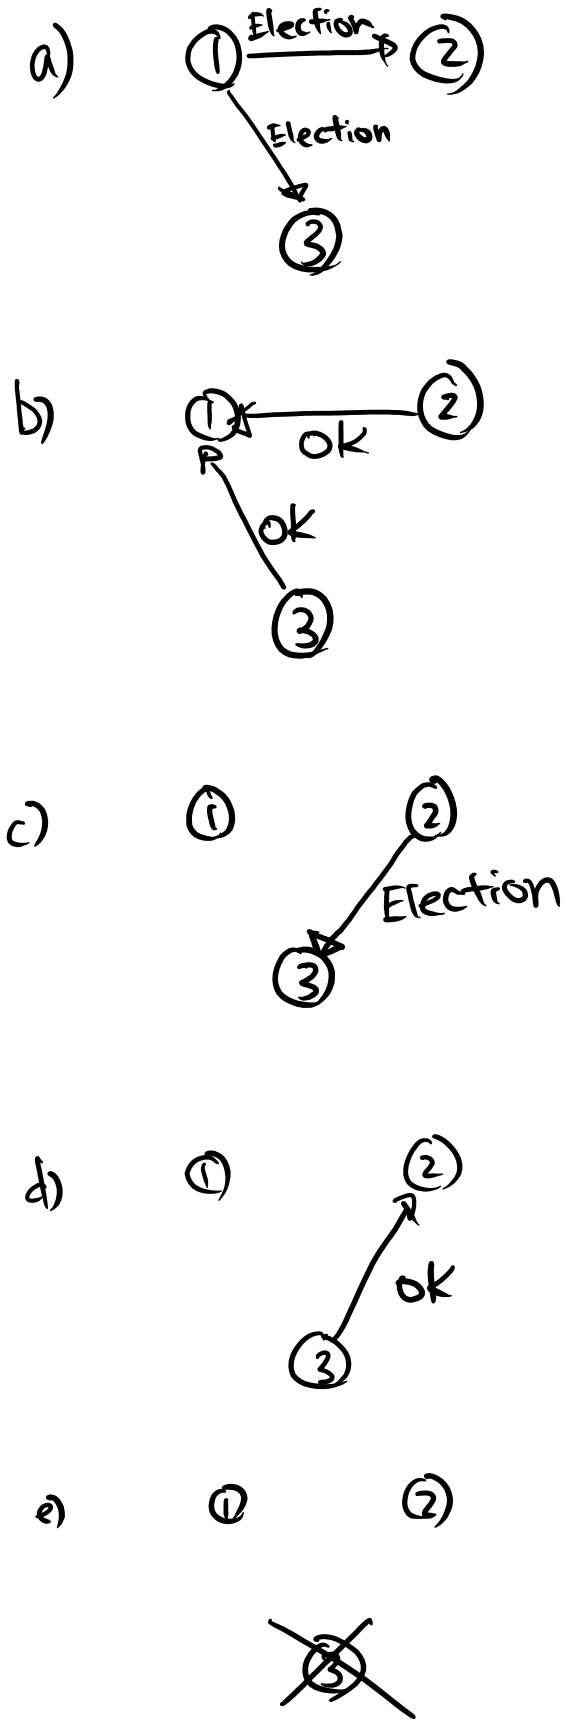
\includegraphics[scale=0.5]{4a}

If failures are allowed during the execution of the algorithm, then it is possible that eventually we make no progress.

\textbf{Progress Property 1:} Eventually some process becomes the leader (wins) and every other process discovers that it is not the leader (loses).

\textbf{Progress Property 2:} If a process does not win then it eventually learns the ID of the leader.

As in the example above, if during step e, the potential leader crashes before it can send out its COORDINATOR message, but after it has sent out its OK message, then no process will become the leader. This breaks \textbf{Progress Property 1}. Because it can't send out its COORDINATOR message, no other processes learn the ID of the leader, because there is no leader. This breaks \textbf{Progress Property 2}.


\clearpage

\item \textbf{Of the three correctness properties described in slide 16, are there any that continue to hold in all possible executions even if processes are allowed to crash during the execution of the algorithm? Give a proof sketch.}

\textbf{Safety property:} There is always at most one leader.

The property that continues to hold in all possible executions, even with a crash is the safety property which states that there is at most one leader.

Let's assume for a contradiction that at some point in the algorithm when a crash occurs, there ends up being more than 1 leaders, which breaks the safety property. 

Let P1, P2 be processes with IDs 1, 2 respectively. 

\textbf{Case 1: Crash on 1st Step}

P1 calls an election, and P1 now crashes. P2 doesn't receive the message. Now, since P1 crashes, it is removed from the elections, and it isn't selected. At this point in time there are no leaders, and since there was no Coordinator message sent, no leader becomes appointed, which contradicts the assumption.

\textbf{Case 2: Crash on 2nd Step}

P1 calls an election, and sends the election message. P2 receives the message, and then crashes before responding. At this point, P1 waits and receives no response, and therefore it becomes the leader. This results in a new leader, and still keeps the safety property since there is at most 1 leader, which happens to be P1.

\textbf{Case 3: Crash on 3rd Step}

P1 calls an election, and sends the election message. P2 receives the message and responds. Now P1 is removed from the election, and P2 is about to become the leader. Before sending off the Coordinator message, P2 crashes. All the other processes haven't received a Coordinator message, and therefore don't know that a new leader has been set. At this point, there are no leaders assigned, and that still holds the safety property, as it states that at most 1 leader exists.

Therefore, a crash at each step still happens to hold the safety property, and therefore contradicts the statement that at some point in the execution of the algorithm the safety property would be violated.


\end{enumerate}


\clearpage

\section{~}

\begin{enumerate}[label=(\alph*)]

\item \textbf{sequentially consistent}

This example is not sequentially consistent.

To have sequential consistency means there must be a total ordering of all operations, and each processor sees its own operations in the same order.

The ordering of P3's operations is R(x)a, R(x)c, R(x)b
The ordering of P4's operations is R(x)a, R(x)b, R(x)c

In the total ordering for all 4 processes, R(x)c must precede R(x)b, or R(x)b must precede R(x)c. So one of P3 or P4's instructions will have to be in a different order, which violates the rules of sequential consistency.


\item \textbf{causally consistent}

\begin{align*}
T1 &= <W(x)a\ \ W(x)c\ >\\
T2 &= <W(x)a\ \ R(x)a\ \ W(x)b\ >\\
T3 &= <W(x)a\ \ R(x)a\ \ W(x)c\ \ R(x)c\ \ W(x)b\ \ R(x)b\ >\\
T4 &= <W(x)a\ \ R(x)a\ \ W(x)b\ \ R(x)b\ \ W(x)c\ \ R(x)c\ >\\
\end{align*}

We see that W(x)a causally precedes R(x)a, which causally precedes W(x)b. W(x)b and W(x)c are both concurrent, so the reads in P3 and P4 are valid under causal consistency, so therefore, this is causally consistent.

\end{enumerate}



\section{~}

A small start-up company is setting up a Cassandra cluster distributed across three data centers: one near Seattle Washington, one near Atlanta Georgia, and one near Frankfurt Germany. Each data object will be replicated three ways, with one copy in each data center.

\begin{enumerate}[label=(\alph*)]

\item \textbf{Suppose that a client application running in the Seattle data center requires a latency bound of $\leq50 ms$ for a Get request. Which of the client-side consistency settings (ONE, QUORUM, ALL) can be used in this particular case assuming no failures? Answer this question using speed of light calculations, assuming that all messages travel at 2/3 the speed of light in a vacuum and that processing delays are negligible.}

The best consistency setting which can be used in this case would be QUORUM. 

Since the distance from Seattle, Washington to Atlanta, Georgia is approximately 3510 km, the time it would take for a request to hit that data center would be the distance divided by $\rfrac{2}{3} c$ where c is the speed of light, so we get:

\begin{align*}
t = \frac{d}{v} = \frac{3510 km}{ \left(\frac{2}{3} \right) \cdot 3 \cdot 10^{8} m/s} \approx 0.01756\ \texttt{seconds} = 17.56\ \texttt{ms} 
\end{align*}

This would result in a round trip of approximately $17.56ms + 17.56ms=35.12ms$, which is less than the $50ms$ latency bound.

If we look at the distance from Seattle to Frankfurt, we see that it is approximately $8203\ km$. If we divide this by $\rfrac{2}{3} c$ where c is the speed of light, we get:

\begin{align*}
t = \frac{d}{v} = \frac{8203 km}{ \left(\frac{2}{3} \right) \cdot 3 \cdot 10^{8} m/s} \approx 0.04104\ \texttt{seconds} = 41.04\ \texttt{ms} 
\end{align*}

So if the latency to get from Seattle to Frankfurt is approximately $41.04\ ms$, then it would take approximately $41.04\ ms + 41.04\ ms =82.08\ ms$ to actually receive the response from the Frankfurt data centre. Therefore, the latency would be over the $50 ms$ bound. 

If we only need a majority to continue, we can use the QUORUM consistency settings so that we only need to have confirmation of writes to the Seattle and Atlanta locations, which will take $35.12\ ms$, which is underneath out bounds, and the application can continue on without waiting for the confirmation of the write to the Frankfurt data centre. 

If we used ALL consistency setting, then we would wait longer than the bound allows, because it would take $82.08\ ms \ge 50\ ms$ to receive a confirmation from the Frankfurt data center. 

Therefore, by using the QUORUM consistency setting, we should still be able to meet our latency requirements.


\item \textbf{Which of the client-side consistency settings ensure that a Get operation can complete even if one data center becomes unavailable?}

The ONE and QUORUM client consistency will ensure that a GET operation can complete even if one data center becomes unavailable. For ONE, as long as we get a response from any of the other data centres that are not down, we can complete a GET request. For QUORUM, since 2 of the 3 data centres are still up, we still can get a majority from the reads and still complete the GET request.

\pagebreak

\item \textbf{What combinations of client-side consistency settings for Get and Put operations can be used to achieve strong consistency (as defined by Werner Vogels) in the absence of failures?}

We can achieve strong consistency as defined by Werner Vogels, $N_R + N_W > N$. Since the QUORUM setting indicates majority, 

\begin{itemize}
\item $N_R$ = ONE, $N_W$ = ALL
\item $N_R$ = QUORUM, $N_W$ = ALL
\item $N_R$ = ALL, $N_W$ = ALL
\item $N_R$ = ALL, $N_W$ = ONE
\item $N_R$ = ALL, $N_W$ = QUORUM
\item $N_R$ = QUORUM, $N_W$ = QUORUM
\end{itemize}

\item \textbf{Suppose that the Atlanta data center becomes unavailable due to a natural disaster. How does your answer to part (a) change?}

Then, since we still have a latency bound of $50\ ms$, we should change our consistency setting to ONE. 

Instead of waiting for a confirmation from a majority of data centers, we only wait for the fastest one to respond. In this case the Seattle data center responds instantly with a latency of $0\ ms$. 

\end{enumerate}

\end{document}
